\chapter{Projekt systemu lokalizacji robota}
\label{ch:system}

W niniejszym rozdziale przedstawiono projekt systemu lokalizacji robota, opartego na znacznikach radiowych. Jego zadaniem jest akwizycja i filtrowanie danych ze znaczników radiowych, konwersja wartości siły sygnału RSSI na odległość, oraz rozwiązywanie zadania lokalizacji na podstawie zebranych danych. 

System akwizycji danych został zaprojektowany w taki sposób, aby możliwe było eksperymentalne porównanie różnych metod lokalizacji. 

\section{Platforma sprzętowa}
\label{sec:hardware}
\subsection{Znacznik radiowy}
\label{subsec:znacznik}

\subsubsection{Protokół}
Znacznik radiowy do wykorzystania w systemie lokalizacji robota winien spełniać szereg wymagań: 
\begin{itemize}
\item \textit{Mały rozmiar} - urządzenie powinno być zwarte i małych rozmiarów, aby możliwe było łatwe umieszczenie go w miejscu pracy robota
 \item \textit{Zasilanie bateryjne} - aby zapewnić swobodę rozmieszczenia, urządzenie powinno być zasilane. Ponadto, aby zapewnić bezobsługowość systemu, czas pracy na baterii powinien wynosić co najmniej 1 rok
 \item \textit{Niski koszt jednostkowy} - system lokalizacji wymaga co najmniej 3 znaczników aby był użyteczny, stąd istotny jest koszt jednostkowy znacznika
\end{itemize}

Do zbioru technologii, jakie pozwalają wypełnić powyższe wymagania, należą m. in. Wi-Fi (por. rozdział \ref{sec:wifi}), ZigBee, Bluetooth wraz z niskoenergetyczną odmianą Bluetooth Low Energy (por. rozdział \ref{sec:bluetooth}). Wszystkie wymienione technologie korzystają z nielicencjonowanego pasma ISM. Technologia ZigBee jest jednak mało popularna, a co za tym idzie - droższa. Technologia Wi-Fi zapewnia duży zasięg, jednakże za cenę wysokiego zużycia energii. 

Protokół Bluetooth w wersji powyżej 4.0, znany pod nazwą Bluetooth Low Energy lub Bluetooth Smart, zapewnia zasięg rzędu 20 metrów przy zachowaniu bardzo niskiego zużycia energii. Istotną zaletą jest to, że układy radiowe BLE są obecne w większości współczesnych smartfonów i laptopów, zaś koszt jednostkowy podstawowego urządzenia BLE wynosi ok 30 zł. Ponadto, istnieją już opracowania dotyczące lokalizacji za pomocą znaczników wykorzystujących Wi-Fi \cite{trilat_iter} oraz klasyczny Bluetooth \cite{trilat_particle}. Wybranie BLE jako protokołu do implementacji pozwala na eksperymentalne sprawdzenie przydatności tego protokołu do lokalizacji, przy jednoczesnym wypełnieniu postawionych wymagań. 

\subsubsection{Moduł BLE}
Do implementacji znacznika wybrano mikrokontroler Nordic Semiconductor nRF51. Jest on oparty o 32-bitowy rdzeń ARM Cortex M0+. W ramach pojedynczego układu scalonego, oprócz procesora, zintegrowano radio 2,4 GHz oraz szereg peryferiów, takich jak liczniki, zegary, interfejsy komunikacyjne czy sprzętowy układ szyfrujący wg algorytmu AES128. Procesor jest taktowany z częstotliwością 16 MHz, ponadto dysponuje oscylatorem o częstotliwości 32 kHz do precyzyjnego mierzenia czasu. Wykorzystany w projekcie wariant mikrokontrolera posiada 32 kB pamięci RAM oraz 256 kB pamięci flash, wykorzystywanej do przetrzymywania programu oraz do dyspozycji aplikacji. 

Podstawową zaletą mikrokontrolera nRF51 jest bardzo niski pobór prądu. W trakcie pracy radia pobiera on ok. 8 mA, natomiast w stanie uśpienia zużycie prądu spada do 2,6 $\mathbf{\mu}$A. Ponieważ czas pracy radia jest o rząd wielkości krótszy od czasu, który procesor spędza w uśpieniu, średnie zużycie prądu wynosi ok 5$\mathbf{\mu}$A i waha się w zależności od skonfigurowanego interwału rozgłaszania \cite{nordic}. 

Jako że niniejsza praca skupia się na zaprojektowaniu oprogramowania i przeprowadzeniu eksperymentów, a nie budowaniu platformy sprzętowej, do projektu wykorzystano gotowy moduł z procesorem oferowany przez sklep Botland (rys. \ref{fig:plytka}). Posiada on, oprócz procesora nRF51822, wszystkie elementy do rozwoju aplikacji Bluetooth, tj. 2 oscylatory kwarcowe, antenę, układ BALUN (BALancer-UNbalancer, konwerter sygnału dla anteny) oraz wyprowadzenie wszystkich nóżek procesora na złącza typu goldpin. Moduł posiada interfejs SWO do programowania i debugowania. Po dołączeniu zasilania (np. koszyczka na baterię CR2032) moduł działa jako samodzielny znacznik (beacon) BLE. Koszt takiego modułu wynosi ok. 30 zł.

Do programowania modułu wykorzystano programator J-Link znajdujący się na płytce rozwojowej nRF52 Developement Kit. 
\begin{figure}
\centering
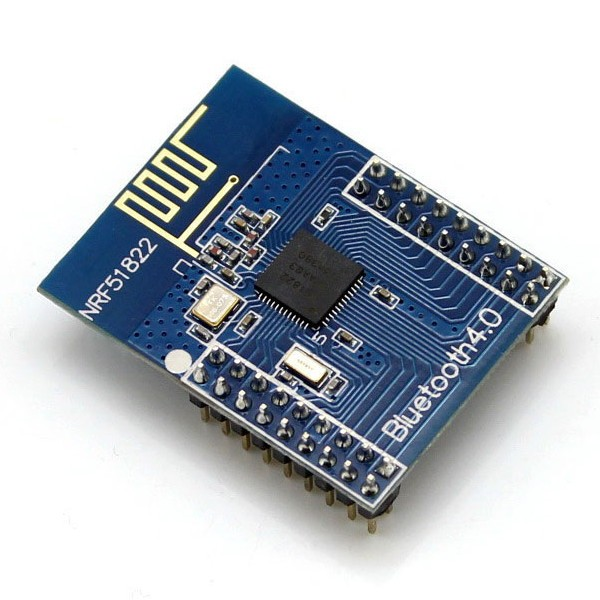
\includegraphics[width=0.7\textwidth]{img/board.jpg}
\caption{Moduł BLE z procesorem nRF51}
\label{fig:plytka}
\end{figure}

\subsubsection{Oprogramowanie znacznika radiowego}
W implementacji oprogramowania znacznika zrealizowano następujące funkcjonalności:
\begin{itemize}
 \item praca w trybie rozgłoszeniowym z interwałem 100 ms,
 \item zawartość pakietu rozgłoszeniowego pozwalająca odróżnić beacon systemu od ewentualnych innych urządzeń BLE w okolicy,
 \item zawartość pakietu rozgłoszeniowego pozwalająca rozróżnić poszczególne beacony wchodzące w skład systemu,
 \item możliwość konfiguracji zawartości pakietu rozgłoszeniowego za pomocą aplikacji mobilnej.
\end{itemize}

Należy zaznaczyć, że zasadnicza funkcjonalność znacznika tj. przekazywanie siły sygnału RSSI jest dostępna dla każdej konfiguracji rozgłaszania, ponieważ jest elementem wbudowanym w stos Bluetooth.

Tabela \ref{tab:adv} opisuje strukturę pakietu rozgłoszeniowego znacznika. Specyfikacja protokołu BLE przewiduje, że w ramce rozgłoszeniowej znajdą się pola reprezentujące poszczególne informacje \cite{ble}. Pole składa się z 2 + N bajtów: pierwszy bajt zawiera długość pola, drugi określa typ informacji, pozostałe zawierają daną informację. Łączny rozmiar wszystkich pól nie może przekroczyć 31 bajtów. Należy także nadmienić, że do długości pola wlicza się bajt typu. Specyfikacja przewiduje typy takie jak nazwa, klasa urządzenia, lista dostępnych serwistów itp.

W ramce znacznika wykorzystano następujące typy (por. tab. \ref{tab:adv}): 
\begin{description}
 \item[Flagi] - pole to jest obowiązkowe w każdej ramce. Zawiera jednobajtowe pole bitowe z flagami określającymi m.in. widoczność urządzenia.
 \item[Nazwa] - pole to zawiera nazwę urządzenia, wyświetlaną przez urządzenia nasłuchujące rozgłaszania (np. smartfon). Nazwa urządzenia to ,,locationTAG''
 \item[Zawartość producenta] - pole to jest przeznaczone do dowolnego wykorzystania przez producenta urządzenia. Zawarto w nim główną informacyjną treść ramki.
\end{description}

Pole ``Zawartość producenta'' zawiera następujące informacje (por. tab. \ref{tab:adv}):
\begin{description}
 \item[Kod producenta] - obowiązkowy kod producenta. Dla producentów niezarejestrowanych w Bluetooth SIG jego wartość wynosi FFFFh
 \item[Identyfikator grupy] - 4-bajtowa liczba całkowita (unsigned int32), służąca do odróżniania grup beaconów (np. zebranych w jednym pomieszczeniu)
 \item[Identyfikator znacznika] - 6-bajtowy identyfikator indywidualny dla znacznika. Jest on równy adresowi fizycznemu MAC znacznika. 
\end{description}


\begin{table}[]
\centering
\caption{Struktura pakietu rozgłoszeniowego}
\label{tab:adv}
\begin{tabular}{|l|l|l|l|l|l|l|l|l|l|l|l|}
\hline
\multicolumn{12}{|c|}{\centering Ramka rozgłoszeniowa [31B]}                                                                                                                         \\ \hline
\multicolumn{3}{|c|}{Flagi [3B]} & \multicolumn{3}{c|}{Nazwa [13B]} & \multicolumn{6}{c|}{Zawartość [15B]}                                                 \\ \hline
\rotatebox{90}{ \textit{Długość} [1B]}   & \rotatebox{90}{\textit{Typ} [1B]}  & \rotatebox{90}{Flagi [1B]}   & \rotatebox{90}{ \textit{Długość} [1B]}      & \rotatebox{90}{\textit{Typ} [1B]}    & \rotatebox{90}{Nazwa [11B]}    & \rotatebox{90}{ \textit{Długość} [1B]}  & \rotatebox{90}{\textit{Typ} [1B]} & \rotatebox{90}{Kod producenta [2B]} & \rotatebox{90}{Identyfikator grupy [4B]} & \rotatebox{90}{Identyfikator znacznika [6B]} & \rotatebox{90}{Wyrównanie [1B]} \\ \hline
\end{tabular}
\end{table}

\subsection{Robot}
W projekcie wykorzystano robota Pioneer 3-AT, będącego na wyposażeniu Laboratorium Robotyki Mobilnej Instututu Automatyki i Robotyki (rys \ref{fig:robot}). Jest to czterokołowy robot o napędzie różnicowym, zaprojektowany jako platforma edukacyjna z szerokimi możliwościami dalszej rozbudowy. Robot w laboratorium został wyposażony w komputer jednopłytkowy Nvidia Jetson TK1, charakteryzujący się dużą mocą obliczeniową i wsparciem przetwarzania równoległego dzięki technologii CUDA. Komputer działa pod kontrolą systemu operacyjnego Ubuntu Linux i wykorzystuje platformę ROS.

Komputer jest połączony z niskopoziomowymi sterownikami sensorów oraz aktuatorów robota za pomocą interfejsu szeregowego RS-232. Ponadto robot posiada kartę Intel Wireless-AC 7260, zapewniającą łączność Wi-Fi oraz Bluetooth, w tym także Bluetooth Low Energy. Układ sensoryczny robota obejmuje enkodery kół, sonar, kamerę USB oraz skaner laserowy Hokuyo URG-04LX-UG01. Do teleoperacyjnego sterowania robotem wykorzystywany jest kontroler z konsoli do gier Xbox \cite{daniel}.

\begin{figure}
\centering
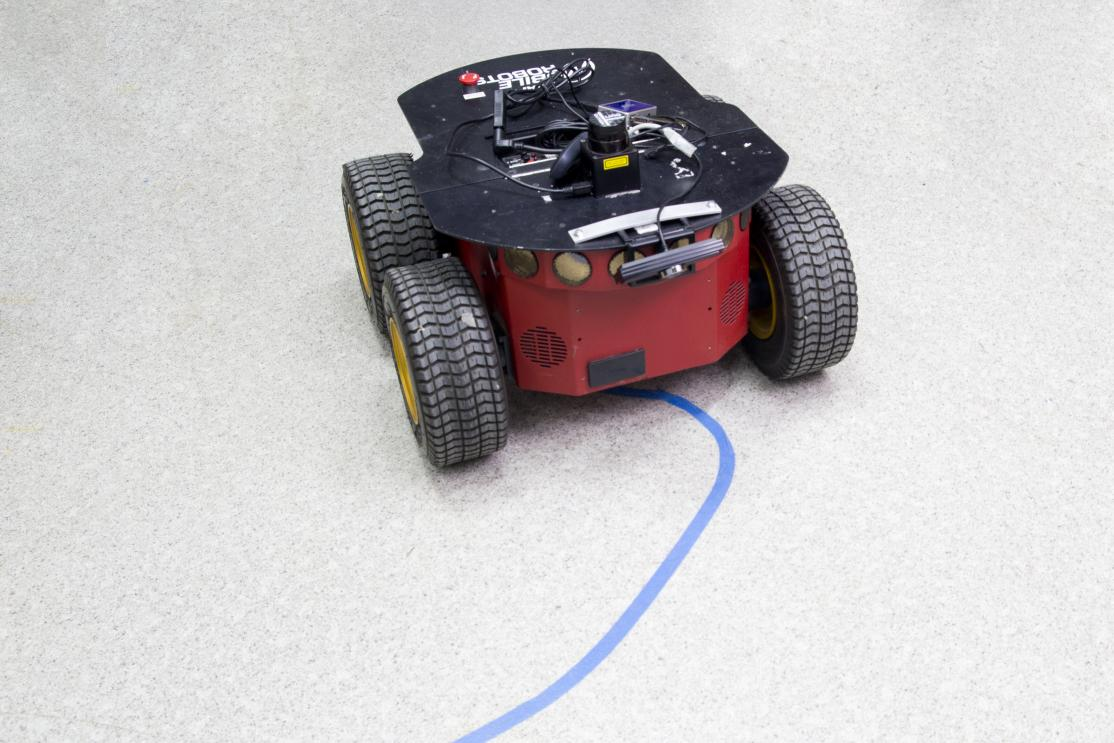
\includegraphics[width=0.7\textwidth]{img/robot.jpg}
\caption{Robot Pioneer 3-AT \cite{daniel}}
\label{fig:robot}
\end{figure}

\section{Oprogramowanie}
Ponieważ robot Pioneer, jak wspomniano powyżej, działa pod kontrolą systemu ROS, zdecydowano zaimplementować oprogramowanie nasłuchujące jako aplikacje ROS. 

ROS umożliwia pisanie aplikacji w trzech językach programowania \cite{roswiki} \cite{learning_ros}: 
\begin{itemize}
 \item C++
 \item Python
 \item JavaScript (Node.js)
\end{itemize}

Język C++ pozwala na napisanie programu bardzo wydajnego obliczeniowo, ponieważ jest to język kompilowany. Jednakże przygotowanie programu i jego zmiany wymagają relatywnie dużego nakładu pracy. 
Język Python, jako język interpretowany, znacznie gorzej radzi sobie w zadaniach obliczeniowych, jednak programy są łatwiejsze do napisania i utrzymania ze względu na prostą składnię, wysokopoziomowość i bogaty zasób bibliotek. Język JavaScript podobnie jak Python, ma przeciętną wydajność obliczeniową. Jednak biblioteki ROS w języku JavaScript zostały zaimplementowane stosunkowo niedawno i można się spodziewać, że zbiór bibliotek jest niekompletny lub niestabilny. 

Ostatecznie, do implementacji aplikacji nasłuchującej wybrano język Python. Wydajność obliczeniowa nie jest problemem, ponieważ aplikacja nie wykonuje żadnych złożonych obliczeń na dużych zbiorach danych. Natomiast elastyczność języka Python pozwoliła na zaprojektowanie aplikacji w taki sposób, aby możliwe było łatwe jej modyfikowanie i rozszerzanie, przy relatywnie niewielkim nakładzie pracy. 


\subsection{Gromadzenie danych ze znaczników}
Gromadzenie danych ze znaczników radiowych jest zadaniem aplikacji nasłuchującej. Nasłuch sensu stricto jest realizowane przez sterowniki stosu Bluetooth systemu operacyjnego. Jednakże zastosowanie danych ze znaczników do lokalizacji wymaga postawienia pewnych dodatkowych założeń:
\begin{itemize}
 \item \textit{Nasłuch ciągły} - większość interfejsów do sterowników Bluetooth udostępnia możliwość skanowania w poszukiwaniu rozgłaszających beaconów przez pewien określony czas, po czym skanowanie jest przerywane. Tymczasem system lokalizacji wymaga, aby skanowanie przeprowadzać w sposób ciągły. Optymalnie, powinno być możliwe przechwycenie każdego pakietu rozgłoszeniowego.
 \item \textit{Filtrowanie urządzeń} -  w środowisku pracy systemu potencjalnie mogą się znaleźć inne urządzenia BLE. Aplikacja nasłuchująca powinna je odfiltrować.
 \item \textit{Interfejsy do dalszego przetwarzania} - zebrane w postaci pakietów rozgłoszeniowych dane powinny być udostępnione do dalszego przetwarzania poprzez odpowiedni interfejs.
\end{itemize}

\subsubsection{Integracja z API Bluetooth}
Ponieważ oprogramowanie ROS działa w systemie operacyjnym Linux, konieczne jest zintegrowanie aplikacji ROS ze sterownikiem Bluetooth.  W większości dystrybucji systemu Linux, Bluetooth działa pod kontrolą stosu BlueZ, będącego oficjalną implementacją stosu Bluetooth dla systemów Linux. 

Do integracji aplikacji w języku Python z API Bluetooth konieczne jest zastosowanie dodatkowej biblioteki. Ponieważ implementacja takiej biblioteki jest zadaniem złożonym i wykraczającym poza zakres niniejszej pracy, wykorzystano bibliotekę bluepy autorstwa Iana Harvey'a. Biblioteka ta stanowi interfejs API BlueZ w języku C do języka Python \cite{pybluez}.

\subsubsection{Architektura aplikacji nasłuchującej}
Tor przetwarzania aplikacji rozłożony jest na dwa wątki wymieniające dane za pomocą chronionej struktury danych. 

API biblioteki BlueZ jest zaprojektowane jako synchroniczne. Oznacza to, że funkcja odpowiedzialna za wykonanie skanowania BLE zwraca dopiero po zakończeniu skanowania. Dlatego, aby zapewnić responsywność programu, skanowanie jest uruchamiane w oddzielnym wątku. Funkcja jest wywoływana w pętli, wykonując skanowanie o zadanej długości. Pętla może być przerwana przez odpowiednią funkcję i wtedy wątek kończy pracę. 
Każde znalezione podczas skanowania urządzenie jest dodawane do kontenera. Kontener jest oparty na mapie (w języku Python nazywanej słownikiem, ang. \textit{dictionary}), w której kluczem jest adres fizyczny MAC beacona, zaś wartością - obiekt przechowujący informacje odebrane z rozgłaszania. Kontener został wzbogacony o dwa dodatkowe mechanizmy: 
\begin{itemize}
 \item \textit{Usuwanie starych wpisów} - wpisy, reprezentujące pakiety rozgłoszeniowe, starsze niż zadana wartość mogą zostać usunięte z kontenera.
 \item \textit{Ochrona dostępu} - dla zapewnienia bezpiecznej synchronizacji między wątkami, każdy dostęp do danych w kontenerze (odczyt, pobranie całej zawartości, dodanie nowego wpisu) jest chroniony za pomocą obiektu \textit{Lock}, zapewniającego atomowość dostępu.
\end{itemize}

W wątku głównym programu prowadzone jest publikowanie wiadomości zawierających dane rozgłoszeniowe. W tym celu aplikacja wykorzystuje obiekt opakowujący klasę \textit{Publisher} biblioteki ROS \cite{agitr}. Jego rolą jest odfiltrowanie urządzeń nienależących do systemu oraz posiadających nieprawidłowy identyfikator grupy (por. \ref{subsec:znacznik}). 

Ustalono, że wszystkie aplikacje systemu będą działać w przestrzeni nazw składającej się z nazwy robota oraz członu \textit{beacon{\_}localization}. Aplikacja nasłuchująca działa pod nazwą \textit{beacon{\_}listener}. Znalezione urządzenia są publikowane do tematu o nazwie \textit{location{\_}tag}. 

\subsection{Filtracja i konwersja danych RSSI na odległość}
\label{subsec:filtracja_rssi}

Jak wspomniano w rozdziale \ref{ch:radio}, wartość siły sygnału RSSI podlega wahaniom nawet w wypadku, gdy nadajnik i odbiornik są nieruchome względem siebie. Ponadto, wahania wartości są dość duże, rzędu 5 dBm. Takie wahanie przekładałoby się bezpośrednio na wahanie przeliczonej odległości i znacznie osłabiało jakość lokalizacji. Dlatego konieczne jest wprowadzenie filtracji wartości siły sygnału, takiej, aby wahania stanu stacjonarnego zostały wygładzone. Jednocześnie bezwładność wprowadzana przez filtr nie może być zbyt duża, ponieważ odbiłoby się to negatywnie na lokalizacji podczas ruchu robota. 

Filtracja i konwersja na odległość jest realizowana przez oddzielną aplikację ROS, noszącą nazwę \textit{rssi2distance}. Aplikacja ta subskrybuje temat \textit{location{\_}tag}, zaś przefiltrowane i skonwertowane dane publikuje w tematach \textit{distances/}$<$nazwa filtra$>$ . Ten sam wynik działania aplikacji jest dostępny również za pomocą usługi ROS działającej pod tą samą nazwą. Dane wynikowe są publikowane w postaci tablicy, zawierającej wszystkie znaczniki radiowe będące aktualnie w zasięgu, łącznie z przefiltrowaną wartością RSSI, przeliczoną odległością oraz pozycją znacznika w układze współrzędnych mapy pomieszczenia.

\subsubsection{Filtracja}
Zaimplementowano następujące filtry (kursywą podano nazwy filtrów używane do nazywania wynikowych tematów i usług):
\begin{enumerate}
 \item \textit{recent} - brak filtra. Filtr zwraca najnowszą znaną wartość RSSI. Jest to najprostsza strategia, używania głównie do testów podczas rozwoju oprogramowania.
 \item \textit{moving{\_}average} - średnia krocząca. Filtr zwraca średnią kroczącą prostą z 5 ostatnich pomiarów:
      \begin{equation}
       \bar P_{k} = \frac{ P_{k} + P_{k-1} + \cdots + P_{k-4} }{5}
      \end{equation}
 \item \textit{probabilistic} - prosty filtr probabilistyczny. Opiera się on na założeniu, że zmiana odległości od znacznika ze stałą prędkością będzie skutkować stałą zmianą wartości RSSI. Działanie filtra można podzielić na fazy estymacji i predykcji \cite{trilat_iter}. Równania estymacji:
 \begin{equation}
  \hat P_{est k } = \hat P_{pred k } + a (P_{k } - \hat P_{pred k })
 \end{equation}
 \begin{equation}
  \hat V_{est k } = \hat V_{pred k } + \frac{b}{T_s} (P_{k } - \hat P_{pred k })
 \end{equation}
 Równania predykcji:
 \begin{equation}
  \hat P_{pred \{k+1\} } = \hat P_{est k } + \hat V_{est k } T_s
 \end{equation}
 \begin{equation}
  \hat V_{pred \{k+1\} } = \hat V_{est k }
 \end{equation}
 
  W powyższych równaniach $\hat P_{est k }$ jest wynikiem działania filtra - wygładzoną wartością RSSI, $V_{est k }$ i $V_{pred k }$ to wartość estymowanego tempa zmiany RSSI, $a$ i $B$ są stałymi strojącymi filtr, zaś $T_s$ jest okresem próbkowania RSSI. 

\end{enumerate}

\subsubsection{Konwersja RSSI na odległość}
Model propagacji, służący do przeliczania RSSI na odległość, również został zaimplementowany na podstawie wzorca Strategii. Model realizuje równanie \ref{eq:logfit_d}.

\subsubsection{Mapa znaczników}
Mapa znaczników jest publikowana przez dodatkową aplikację o nazwie \textit{beacon{\_}tf{\_}publisher}. Pobiera ona konfigurację mapy w postaci koordynatów i odpowiadających im identyfikatorów znacznika z pliku YAML, następnie publikuje w postaci transformacji z układu współrzędnych mapy do układów poszczególnych znaczników, wykorzystując bibliotekę \textit{tf}. 


\subsection{Trilateracja}
Dysponując oprogramowaniem do zbierania danych ze znaczników i konwersji siły sygnału RSSI na odległość, przystąpiono do projektowania właściwych aplikacji lokalizujących. Pierwsza z nich wykorzystuje technikę trilateracji. 
Strukturę aplikacji rozwiązującej zadanie trilateracji oparto na pętli wykonującej się z określonym interwałem. W każdej iteracji wykonywane jest zapytanie do usługi ROS udostępnianej przez aplikację \textit{rssi2distance}. W odpowiedzi otrzymywana jest lista znaczników znajdujących się w zasięgu, wraz z przefiltrowaną wartością RSSI, przeliczoną wartością odległości i pozycją znacznika w układzie mapy. Możliwy jest wybór metody filtracji za pomocą odpowiedniego parametru na serwerze parametrów ROS. 

Jeśli w danej iteracji w zasięgu znajdowało się co najmniej trzy znaczniki, wykonywane jest rozwiązanie zadania trilateracji. Dostępne są dwie, bardzo zbliżone metody trilateracji:
\begin{enumerate}
 \item \textit{metoda Newtona} - opisana w rozdziale \ref{sec:trilateracja}
 \item \textit{metoda L-BFGS (Limited-Memory Broyden–Fletcher–Goldfarb–Shanno } - jest to metoda minimalizacji należąca do rodziny metod quasi-Newtonowskich, implementowana przez bilbiotekę \textit{scipy}
\end{enumerate}
Metoda trilateracji również może być wybierana za pomocą serwera parametrów. 

Wynik obliczeń jest konwertowany na wiadomość typu \textit{geometry{\_}msgs/Pose}), reprezentującą pozycję i orientację obiektu w przestrzeni trójwymiarowej. Jest to typowa konwencja w systemie ROS, nawet jeśli lokalizacja ogranicza się do dwóch wymiarów. Wynik jest publikowany w temacie \textit{beacon{\_}localization/bl{\_}pose} oraz jako transformacja z układu mapy do układu robota. 


\section{Filtr cząsteczkowy}
Ponieważ algorytm trilateracji wykorzystuje tylko dane ze znaczników, jest wrażliwy na zakłócenia wynikłe z ich działania, np. rozrzut wartości RSSI w stanie ustalonym. Dlatego następnym krokiem było zaprojektowanie aplikacji lokalizującej robota w oparciu nie tylko o dane ze znaczników, ale także z sensorów odometrycznych. W celu zintegrowania tych danych wykorzystano filtr cząsteczkowy, co do teorii opisany w rozdziale \ref{sec:filtr-czasteczkowy}.
Filtr cząsteczkowy zaimplementowano w oparciu o implementację autorstwa Dakoty Nelsona dostępną na licencji MIT. Źródłowa implementacja dotyczyła filtra cząsteczkowego wykorzystującego skaner laserowy oraz sensor odometryczny. Aplikacja subskrybuje do tematu \textit{distances/}$<$nazwa filtra$>$, gdzie publikowane są tablice znajdujących się w zasięgu znaczników, wraz z ich pozycjami na mapie. Aby ograniczyć obciążenie komputera obliczeniami, algorytm filtra jest wykonywany tylko jeśli przemieszczenie kątowe lub liniowe robota wynikłe z pomiaru odometrycznego przekroczyło pewien konfigurowalny próg. Jako metodę resamplingu wykorzystano algorytm SRR (\textit{Sequential Random Resampling}, ang. sekwencyjny losowy resampling) \cite{jupyter}.